
\documentclass[12pt]{article}


\usepackage{graphicx, url}
\usepackage[utf8x]{inputenc}
\usepackage[french]{babel}
\usepackage[T1]{fontenc}
\usepackage[english=american]{csquotes}
\usepackage{float}
\usepackage{comment}
\usepackage{amsmath}
\usepackage{amssymb}
\usepackage{enumerate}
\usepackage{subcaption}
\usepackage{setspace}
\usepackage{tabularray}
\usepackage{subcaption}
\usepackage{layout}

\usepackage[style=abnt]{biblatex}

% indica o arquivo com as referencis bibliograficas
\addbibresource{}

\title{Optimisation du moment et de la fréquence d'injection de traitement pour les gliomes de bas grades chez l'adulte} % titulo

\author{Maia COLLIN, Paul HENTON, Ambre JAEGER} % autor principal, orientador

\usepackage{fancyhdr}
\usepackage{geometry}
\usepackage{hyperref}
\usepackage{color} 
\hypersetup{
unicode=true,
pdfauthor={},
pdfkeywords={},
pdftitle={},
pdfsubject={},
pdfstartview={FitV}, 
    colorlinks,%
    citecolor=blue,%
    filecolor=blue,%
    linkcolor=red,%
    urlcolor=blue
}

\geometry{hmargin=2cm, vmargin=2cm }

\pagestyle{fancy}
\fancyhf{}
\rfoot{}
\lhead{\textbf{\large TP Modélisation  - M2 2024}}
\rhead{\textbf{\large M. Collin, P. Henton, A. Jaeger}}


% %%%%%%%%%%%%%%%%%%%%%%%%%%%%%%%%%%%%%%%%%%%%%%%%%%%%%%%%%%%%%%

\begin{document}
\maketitle % Não remova essa linha!
     
\section{Introduction}
Que sont les gliomes de bas-grades leurs propriétés ?\\
Quels sont les traitements existants?\\
Question scientifiques: \textbf{Quels sont les temps et fréquences optimales d'administration du traitement pour maximiser leur efficacité ?}


\section{Etude du modèle}
\subsection{Présentation du modèle}
\begin{figure}
    \centering
    \begin{subfigure}[t]{0.45\textwidth}
        \centering
        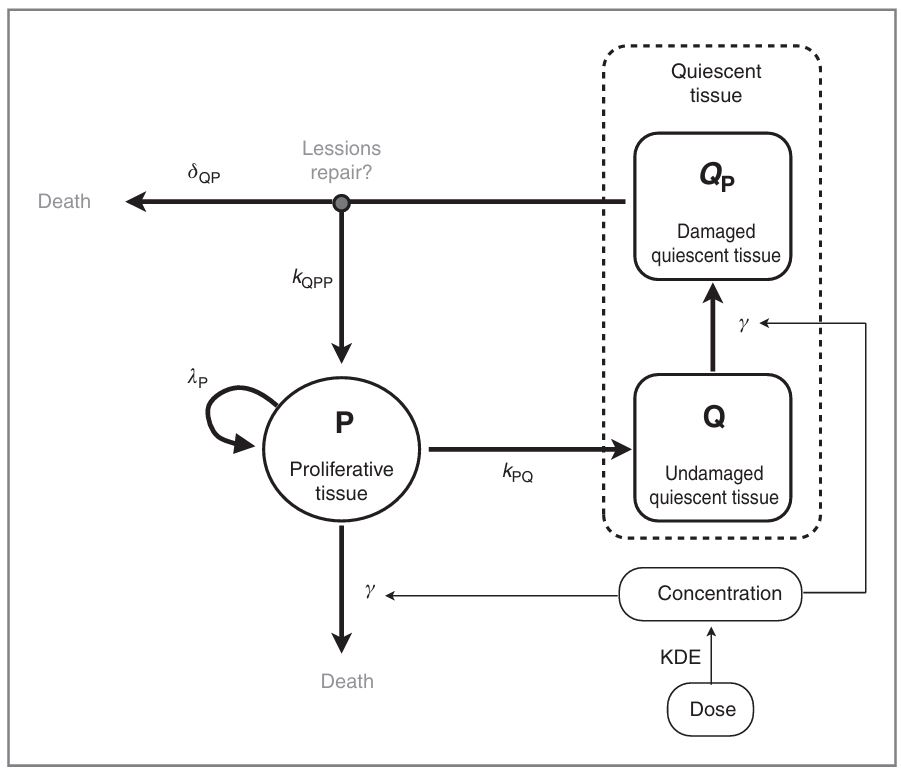
\includegraphics[width=\linewidth]{Image/modele.JPG} 
        \caption{} \label{fig:model}
    \end{subfigure}
    \hfill
    \begin{subfigure}[t]{0.45\textwidth}
        \centering
        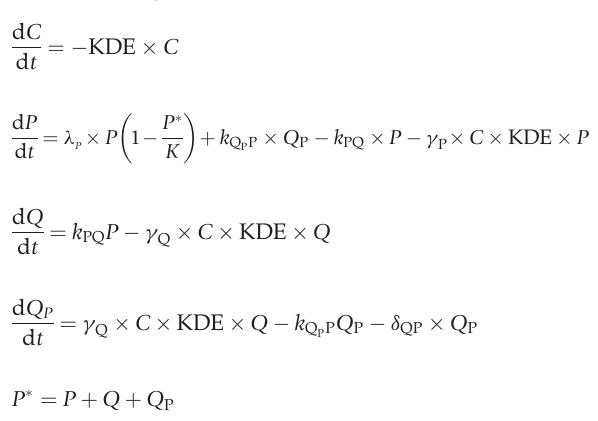
\includegraphics[width=\linewidth]{Image/eq.JPG} 
        \caption{} \label{fig:teq}
    \end{subfigure}

    \vspace{1cm}
    \begin{subfigure}[t]{\textwidth}
    \centering
        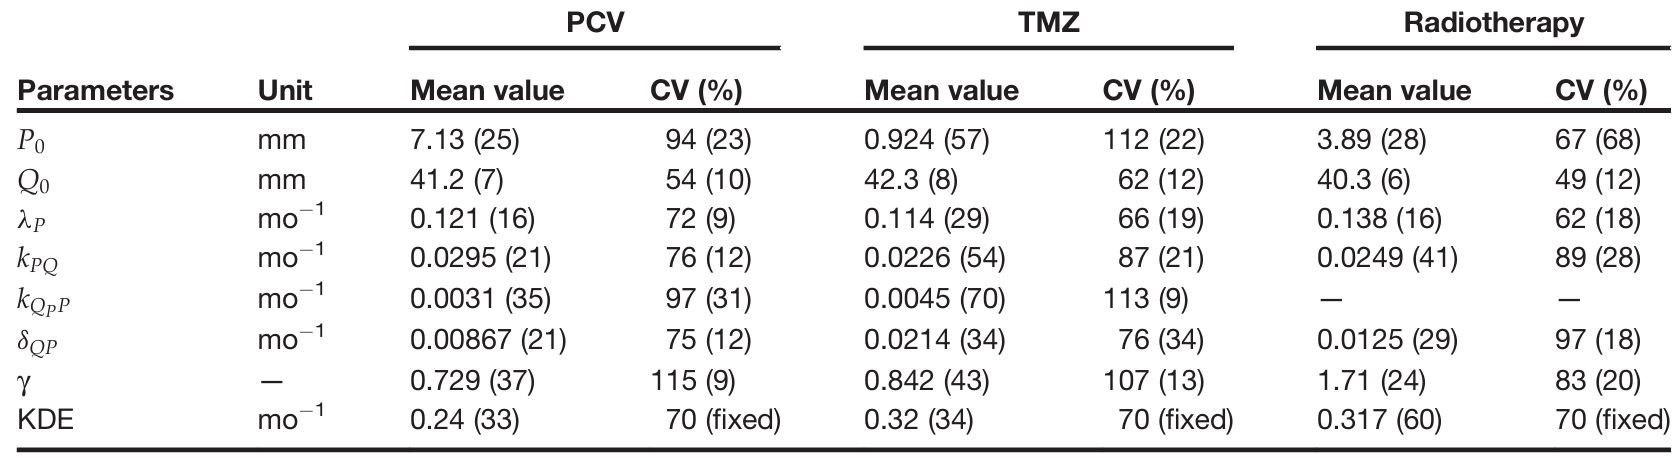
\includegraphics[width=\linewidth]{Image/tableau.JPG} 
        \caption{} \label{fig:tableau}
    \end{subfigure}
    
    \caption{\textbf{Présentation du modèle \cite{} (a).} Modèle à 3 compartiments $P$ (tissu prolifératif), $Q$ (tissu quiescent), $Q_{p}$ (tissu quiescent endommagé). Sous l'effet du traitement de concentration C (normalisée) qui va endommagé l'ADN des cellules, P peut être endommagé et mourir selon efficacité $\gamma$ et Q peut devenir $Q_p$ selon efficacité $\gamma$. $Q_{p}$ mourrir selon $\delta$ ou redevenir prolifératif. Les coefficients $k$ désigne la proprtion de tissu qui transitionne vers un autre état.  \textbf{(b).} Mise en équation du modèle proposé. \textbf{(c).} Estimation des paramètres d'après fitting de données de patients ayant subi les différents traitements au modèle. CV désigne le coefficient de variation qui caractérise la variabilité interindividuelle. L'erreur sur les estimations est donnée par les nombres entre parenthèses en pourcentage. Pour plus de précisions se référer à l'article référence\cite{}}
\end{figure}

\subsubsection{Explication du modèle}
\subsubsection{Paramétrisation}
Dans l'article de référence, des données de patients ayant été traité par différentes thérapies: Chimiothérapies PCV, Chimiothérapies TMZ et radiothérapies; ont été utilisées pour paramétriser le modèle. Pour chacune de ces cohortes ils ont estimé des paramètres moyens et quantifier la variabilité interindividuelle par le coefficient de variation (CV) \ref{fig:tableau}.  On constate que pour les différents traitements, le DT évolue différemment \ref{fig:evol_moy}. $\lambda_{p}$ (coefficient de croissance du tissu), $P_{0}$ (tissu prolifératif à l'instant 0) et $Q_{0}$ (tissu quiescent à l'instant 0) sont des paramètres associés à la tumeur.  Ces paramètres peuvent être estimées sur les patients avant le début du traitement. On estime souvent P égal à 10\% du DT et on peut mesurer $\lambda_{p}$ sur la croissance de la tumeur pendant le pré-traitement. Une estimation individuelle du modèle permet de prédire avec plus de précision l'évolution du DT de la tumeur avec le modèle. En effet, ces paramètres notamment $\lambda_{p}$ varient beaucoup entre individus\ref{fig:tableau}. Or, comme on le constate des faibles variations de ces paramètres sont suffisantes pour modifier significativement  l'évolution du DT \ref{fig:rand_traj}. On fait varier $P_{0}$ entre 3 et 15\% (variation observées dans les différentes cohortes) du DT et on fait varier $\lambda_{p}$ selon sa distribution donnée pour le traitement PCV \ref{fig:tableau}. On observe des trajectoires très différentes.  On  souhaite comprendre le rôle de ces différents paramètres sur l'évolution du DT. De même, les caractéristiques du traitement, $\gamma$, $C$ vont influer sur l'évolution de la tumeur. On va donc explorer l'espace des paramètres pour évaluer l'influence de ces différents paramètres.  
\begin{figure}
    \centering
    \begin{subfigure}[t]{0.45\textwidth}
        \centering
        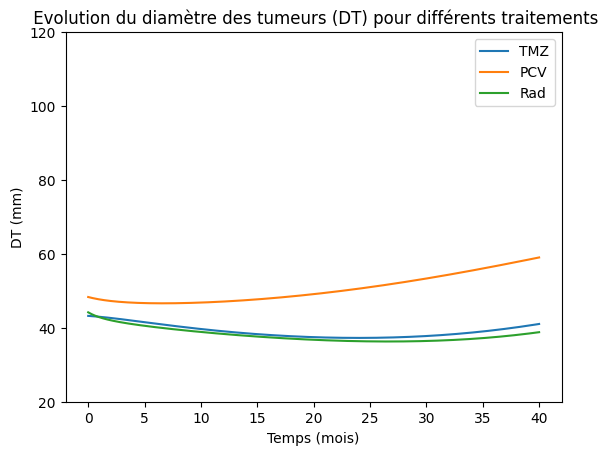
\includegraphics[width=\linewidth]{Image/evolution_TD_param_moy.png} 
        \caption{} \label{fig:evol_moy}
    \end{subfigure}
    \hfill
    \begin{subfigure}[t]{0.45\textwidth}
        \centering
        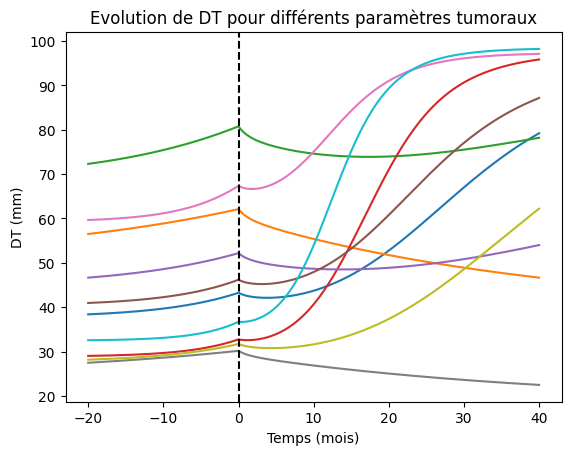
\includegraphics[width=\linewidth]{Image/ex_traj.png} 
        \caption{} \label{fig:rand_traj}
    \end{subfigure}

    \caption{\textbf{(a).} Evolution du diamètre d'une tumeur (DT) pour les paramètres de populations moyens des trois traitements chimio thérapie PCV, TMZ ou radiothérapie \cite{}. \textbf{(b).} Evolution du DT pour les paramètres moyens PCV sauf $\lambda_{p}$, $P_{0}$, $Q_{0}$ choisi aléatoirement selon les distributions les valeurs moyennes et coefficient de variation indiqué dans \ref{fig:tableau} }
\end{figure}

\subsection{Exploration de l'espace des paramètres}
On constate que des variations de ces paramètres modifient significativement l'évolution du DT \ref{fig:rand_traj}.  

\begin{figure}
    
    \begin{subfigure}[t]{\textwidth}
    \centering
        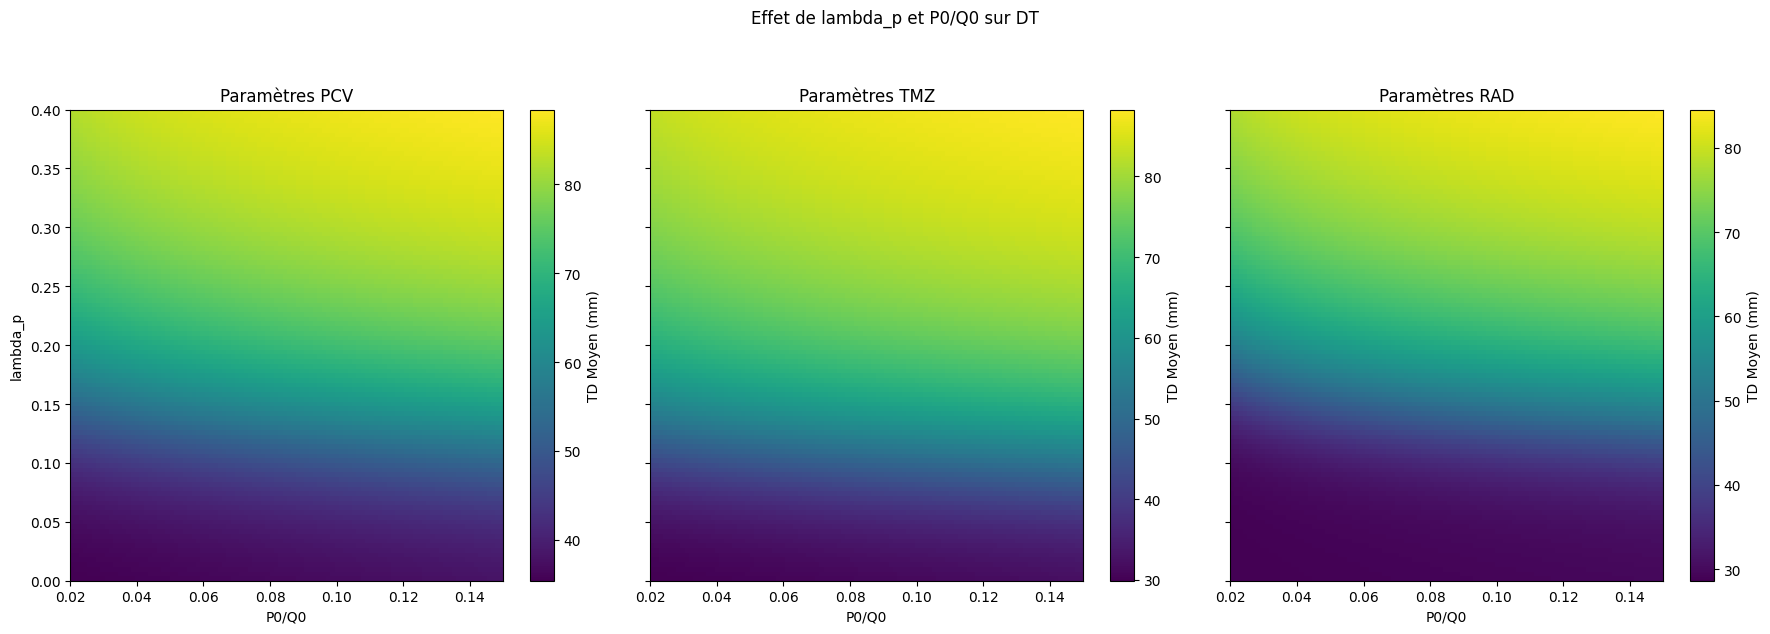
\includegraphics[width=\linewidth]{Image/heatmap_lambdap_p0Q0.png} 
        \caption{} \label{fig:heatmap}
    \end{subfigure}
    \vspace{1cm}
    \centering
    \begin{subfigure}[t]{0.45\textwidth}
        \centering
        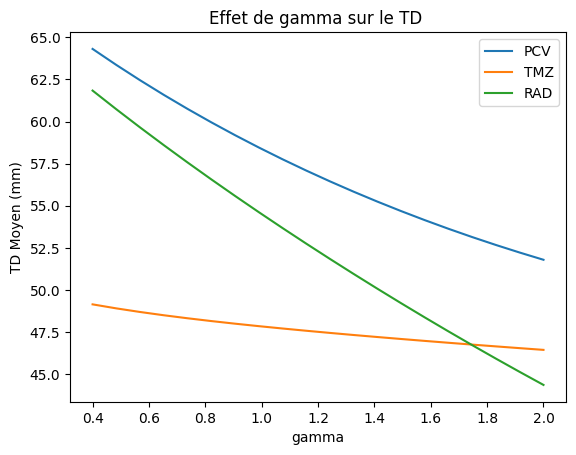
\includegraphics[width=\linewidth]{Image/effet_gamma.png} 
        \caption{} \label{fig:effet_gamma}
    \end{subfigure}
    \hfill
    \begin{subfigure}[t]{0.45\textwidth}
        \centering
        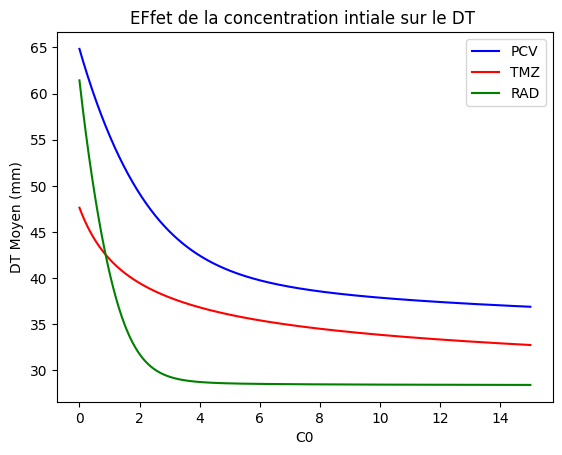
\includegraphics[width=\linewidth]{Image/effet_C.png} 
        \caption{} \label{fig:effet_C}
    \end{subfigure}

    \caption{\textbf{(a).} Effet de $\lambda_{p}$ et $\frac{P_{0}}{Q_{0}}$ sur le DT moyen, jaune indique un DT grand et bleu faible. \textbf{(b).} Effet de $\gamma$ sur le DT, les autres paramètres sont choisis selon les valeurs moyennes des traitements. \textbf{(c).} Effet de $C$ sur le DT, les autres paramètres sont choisis selon les valeurs moyennes des traitements.}

\end{figure}

\section{Optimisation du moment et de la fréquence d'injection}
\subsection{Optimisation pour une unique injection}

\begin{figure}

    \centering
    \begin{subfigure}[t]{\textwidth}
        \centering
        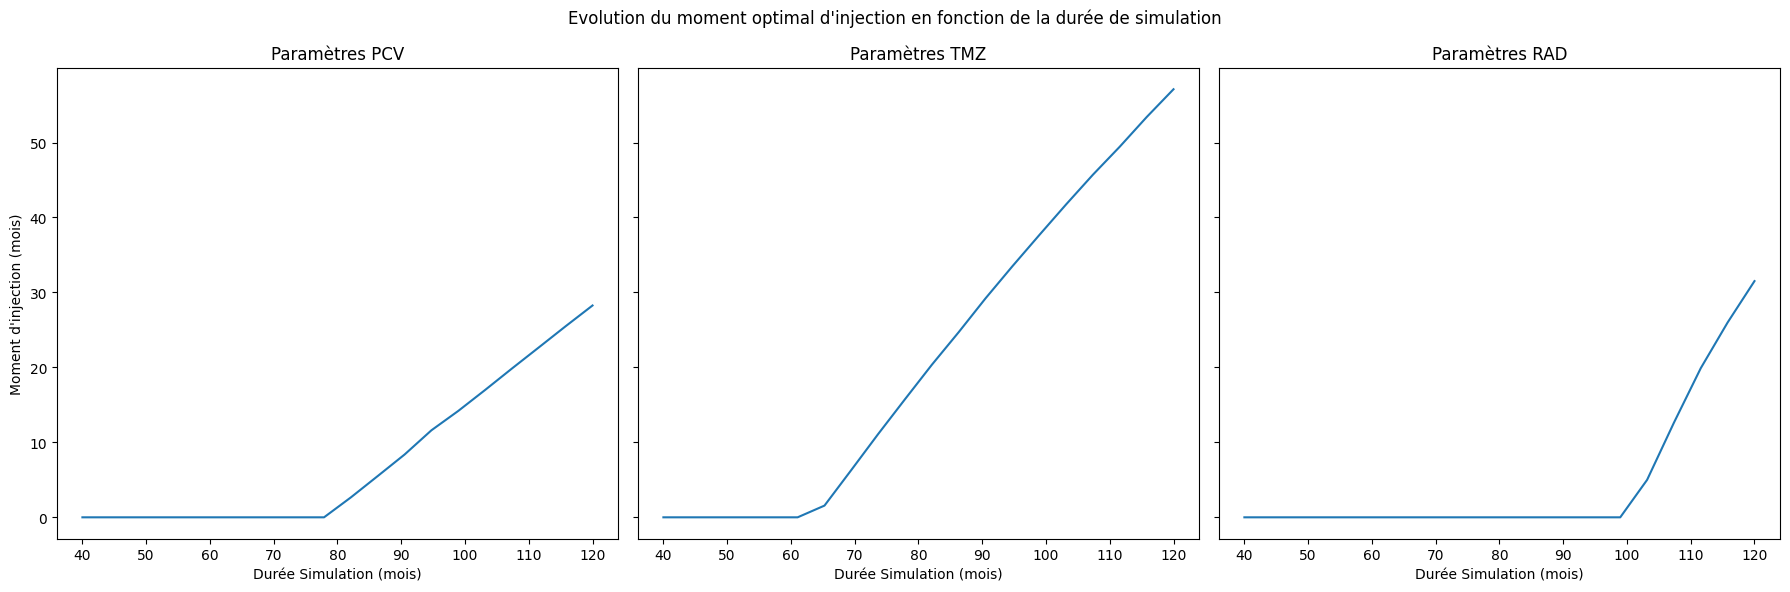
\includegraphics[width=\textwidth]{Image/duree_simu.png} 
        \caption{} \label{fig:duree_simu}
    \end{subfigure}

    \vspace{0.5cm}

    \begin{subfigure}[t]{\textwidth}
        \centering
        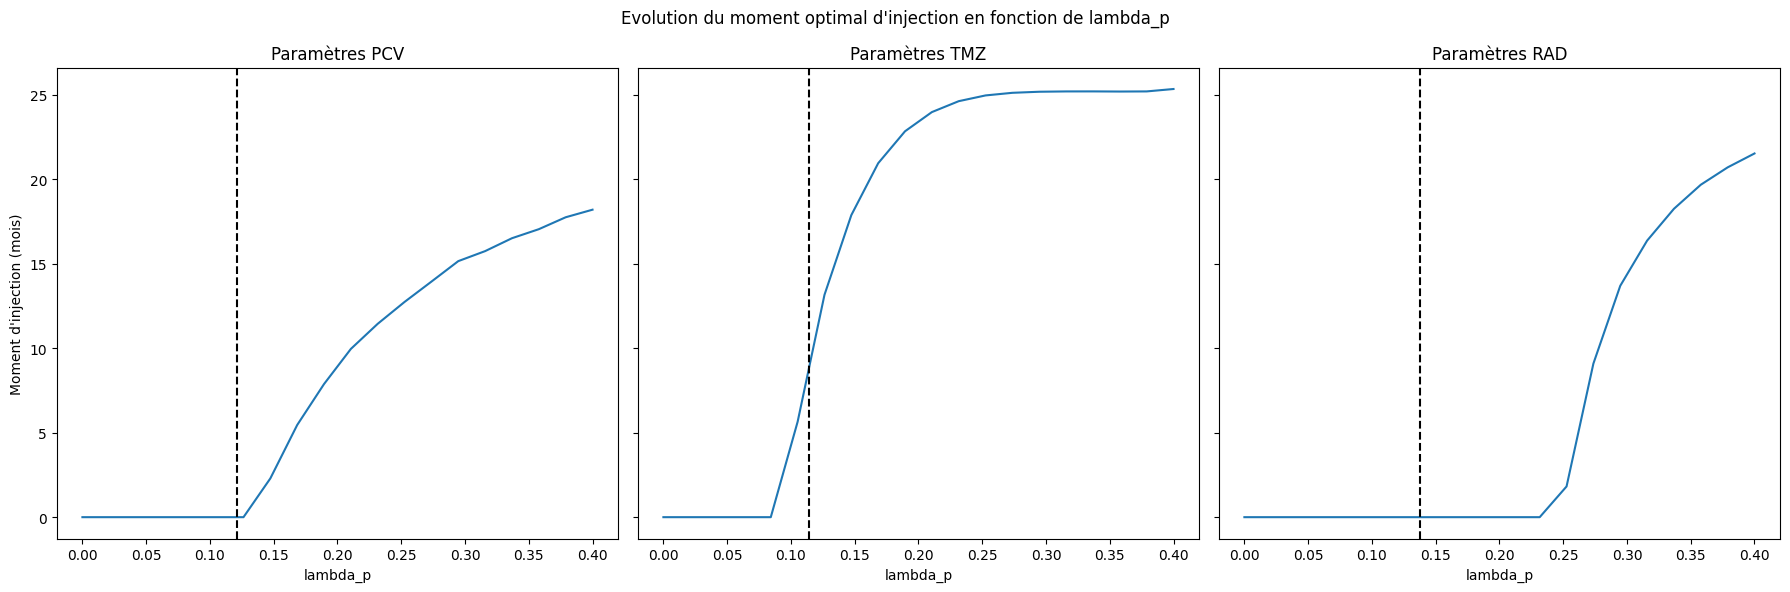
\includegraphics[width=\textwidth]{Image/effet_lambda_moment.png}
        \caption{} \label{fig:effet_lambda_moment}
    \end{subfigure}

    \caption{\textbf{(a).} DT moyen pour des simulations de durée entre 20 et 120 mois pour les paramètres moyens des différents traitements. \textbf{(b).} Effet de $\lambda_{p}$ sur le DT pour une durée de simulation de 40 mois.}
\end{figure}

\section{Conclusion}
\subsection{Limites}
\subsection{Perspectives}

\end{document}